\noindent La phase d'adaptation sera initiée si le temps le permet, et s'il est jugé bon d'améliorer la qualité de la segmentation. Il y a deux types d'adaptation possible: matérielle et logicielle.
\vspace{\baselineskip}
\\
\noindent L'adaptation matérielle sera jugée nécessaire si le nano ordinateur ne peut être utilisé tel quel pour répondre aux objectifs. Par exemple si le nano ordinateur devient non utilisable (lent ou sans réponse) après un certain temps. La stratégie sera de diagnostiquer le comportement et d'évaluer un remède. L'une des pistes de solution privilégiée sera de lui apporter plus de puissance, comme de l'ajout de mémoires ou un espace de stockage plus performant. Plus complexe, optimiser le processus, par exemple certains traitements, serait aussi une option.
\vspace{\baselineskip}
\\
\noindent L'adaptation logicielle, quant à elle, sera jugée nécessaire si la prédiction de la segmentation est en deçà des attentes, ou inutilisable. Le choix d'adapter un modèle avec les méthodes de "Transfer Learning" et "Domain adaptation" sera la première option privilégiée, car cela procure un gain de temps non négligeable: il n'y a pas besoin de passer à travers tout le processus "essai-erreur", couteux en temps, en énergie et en ressources matérielles, d'apprentissage et de paramétrisation du modèle. Des efforts conséquents seront par contre nécessaires pour générer les images vérités terrain \acrshort{gt} avec le jeu de données local, celui de l'\acrshort{apcpontjc} de préférence, personnel ou autre sinon.
\vspace{\baselineskip}
\\
\noindent Le diagramme de la figure \ref{fig:metho_adaptation} présente la méthodologie qu'il faut suivre pour adapter un modèle à un nouveau jeu de données et à une autre résolution. La première étape est de sélectionner un modèle déjà entrainé et qui semble pouvoir être le meilleur candidat pour aider à répondre à la problématique. C'est un travail de recherche et de test minutieux, qui est le plus important de toutes les étapes. La seconde activité est conséquente en efforts: préparer le jeu de données, incluant les images vérité terrain, les bonnes résolutions; et déterminer les classes et la palette de couleurs nécessaires. L'étape suivante est d'étudier l'architecture du modèle, afin de l'adapter au jeu de données, aux classes, et au besoin modifier les couches de l'architecture afin d'avoir une segmentation la plus précise et fine possible. Une fois ces étapes de préparation complétées, le ré entrainement du modèle peut s'effectuer, et la segmentation évaluée. Cette phase d'adaptation est un processus itératif, qui peut être représenté par la figure \ref{fig:methodologie_complexe_realiste}.
\label{metho_adaptation}
\begin{figure}[H]
    \centering
    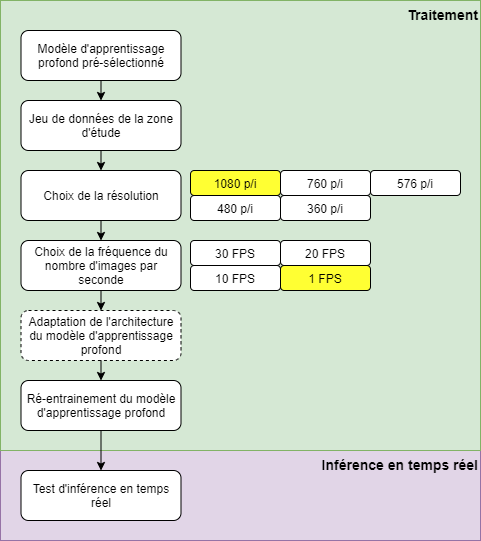
\includegraphics[width=0.65\textwidth]{metho_traitement_eval.png}
    \caption{Méthodologie du traitement et adaptation}
    \label{fig:metho_adaptation}
\end{figure}